%
% Chapter 1
%

\chapter{Introduction}

% What is matter?
Visible matter comprises $\sim$5 percent of the universe. This matter makes up all living things and ecosystems, including the stars and planets. This matter exists entirely within the atom, with the nucleus holding more than 99.9 \% of all matter. The nucleus is comprised of protons and neutrons in different configurations, held together by the strong force. Understanding this essential building block of the universe is at the heart of understanding how matter is formed and evolves.

The periodicity of phenomena on the atomic level and higher is well documented near stability, from the lattice structures of crystals, to the periodic table of the elements, organized in a way that groups elements that behave similarly due to the structure of the orbiting atomic electrons. But, this periodic table does not delve into the subatomic level. The periodic table separates out atoms by the number of protons, which equates with the atomic number, but the number of neutrons in a nucleus can also vary. When mapping these two, we create Figure \ref{fig:chart}, known as the chart of nuclides. These nucleons are held together by the strong force, which has a short range. In the low-mass region of the chart, this creates a linear trend for the line of stability. As mass and the total number of nucleons increases, the line of stability trends toward the neutron side, due to repulsion by the coulomb force in the protons. As the neutrons do not contribute significantly to the coulomb force, the addition of more neutrons creates larger separation between protons, decreasing the coulomb contribution.

\begin{figure}
    \centering
    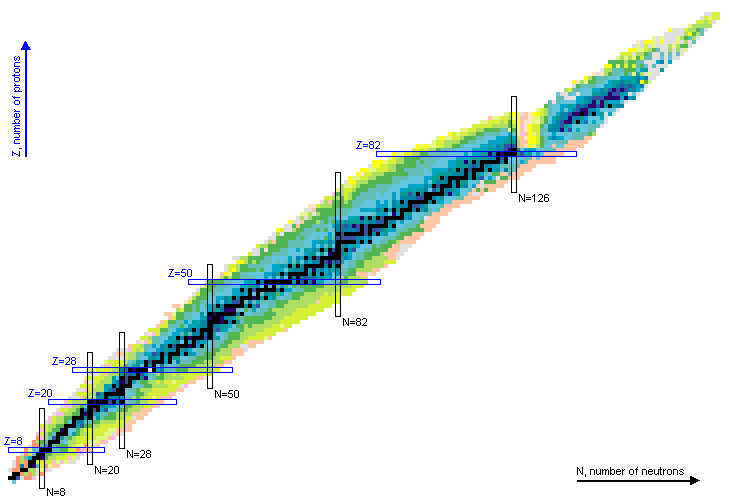
\includegraphics[scale=0.5]{Introduction_Figs/chartofnuclides_nndc.png}
    \caption{The chart of nuclides. The $x$-axis is increasing in neutron number from left to right, and the $y$-axis is increasing in proton number from bottom to top. The lower leftmost corner is the lightest elements, while the upper right are the heaviest, including superheavy elements. Black boxes indicate stable nuclei. These nuclei are in the "center" of the chart, and known colloquially as the valley of stability. To either side of these stable nuclei are radioactive nuclei, which become shorter lived the farther they are from the valley, indicated by the lightening color. The lines marked at 2, 8, 20 etc. are the closed shells for spherical nuclei, and are discussed in further depth within the text. Taken from \citep{nndc:_chart}.}
    \label{fig:chart}
\end{figure}

The chart of nuclides has several notable features in this form. The color coding in Figure \ref{fig:chart} is representative of the lifetimes of the isotopes represented in each box: lighter boxes are shorter-lived, while darker boxes are longer lived, with black boxes being stable isotopes. This creates a black line going up at approximately $N=Z$, known as the valley of stability. Additionally in this figure, several rows and columns are singled out. These rows and columns are a series of numbers referred to as the "magic" numbers, and highlight a form of periodicity in nuclei. 

This periodic nature is explained through the shell model. Based on the same idea as atomic electrons, the "shells" occur due to the energy gap in levels. The neutrons and protons each have separate potential wells and levels populated. When examining solutions to this potential well, the magic numbers naturally form after including angular momentum, and taking the spin-orbit interaction into account, as seen in Figure \ref{fig:shellmodel}. These magic numbers represent closed shells of a spherical nucleus model. It is of note, that a doubly-magic nucleus, that is, a nucleus with both neutron and proton close shells, is spherical. However, a nucleus with only a single closed shell is not, necessarily, spherical. These closed shells cause a variety of effects, including high energy of the first excited $2^+$ state at closed shells, seen in Figure \ref{fig:E2bymass}. The high energy of the first excited $2^+$ state near the closed shells is due to the large energy gaps that occur at closed shells, seen on the right side of Figure \ref{fig:shellmodel}.
 %, and the low reduced transition rate between this first excited state and the ground state, seen in Figure \ref{fig:reducedtrans}. 

\begin{figure}
    \centering
    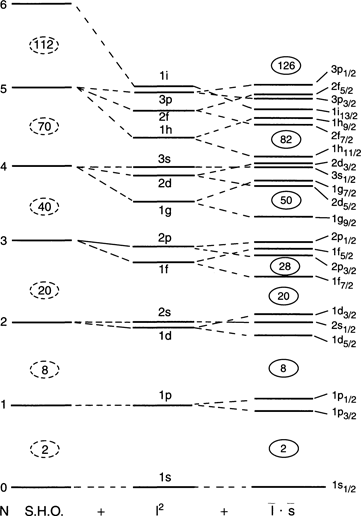
\includegraphics[scale=2]{Introduction_Figs/ShellBreakdownCasten.png}
    \caption{The evolution of the shel model and the creation of the closed shells of a spherical nucleus. On the left is the spherical harmonic oscillator. By adding in an angular momentum term, some of the degenerate levels separate. By further adding a spin-coupling term, the levels separate with energy spacings that create the closed shells and the magic numbers. Taken from \citep{casten90:_structure}.}
    \label{fig:shellmodel}
\end{figure}

\begin{figure}[!tbp]
    \centering
    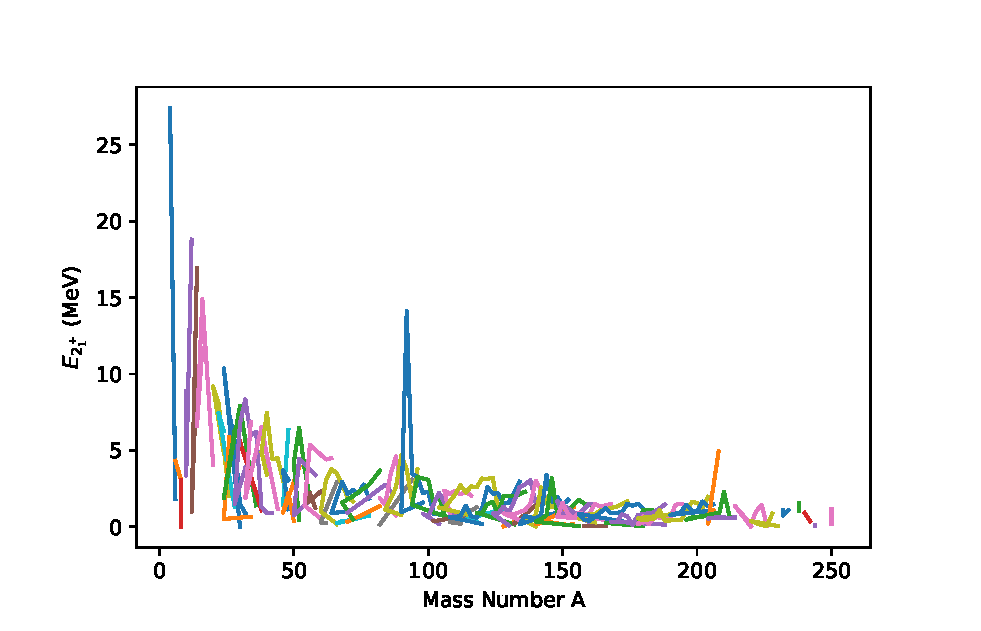
\includegraphics[scale=0.9]{Introduction_Figs/E2vsA.eps}
    \caption{The energy of the first excited $2^+$ state, plotted in isotopic chains by mass, distinguished by color. Areas of high excitation energy, around A$\sim$90,140,210 all correspond to doubly magic areas. The areas around A$\sim$110,170 have much lower excitation energies and correspond to areas of deformation. }
    \label{fig:E2bymass}
\end{figure}

% \begin{figure}
    \centering
    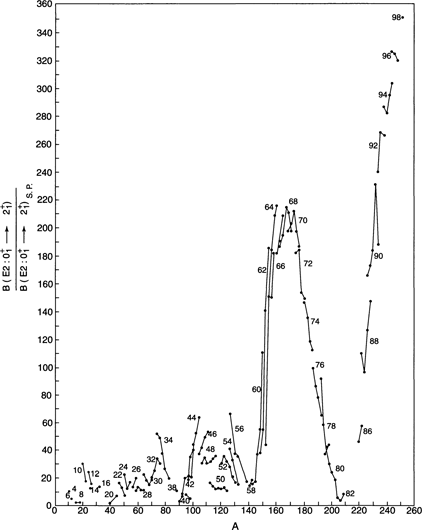
\includegraphics[scale=2]{Introduction_Figs/ReducedTransbyMassCasten.png}
    \caption{A plot of the reduced transition rate between the first excited $2^+$ state and the ground state in even-even nuclei, in single particle units. Areas of low rates, around A$\sim$90,140,210, correspond to closed shells, while the areas around A$\sim$110,170,250, have much higher rates, and correspond to deformed nuclei. Taken from \citep{casten90:_structure}.}
    \label{fig:reducedtrans}
\end{figure}

Outside of these closed shells, there are large regions that do not work within the paradigm created by this phenomenon. Nuclei near the close shells are generally spherical in nature. However, the shell model breaks down far from the closed shells. In some cases, the magic numbers themselves appear to change. This change can be charted using the Nilsson model, which shows the evolution of the levels in the shell model as a function of the deformation parameter $\beta$, see Figure \ref{fig:nilsson}.

\begin{figure}[!tbp]
    \centering
    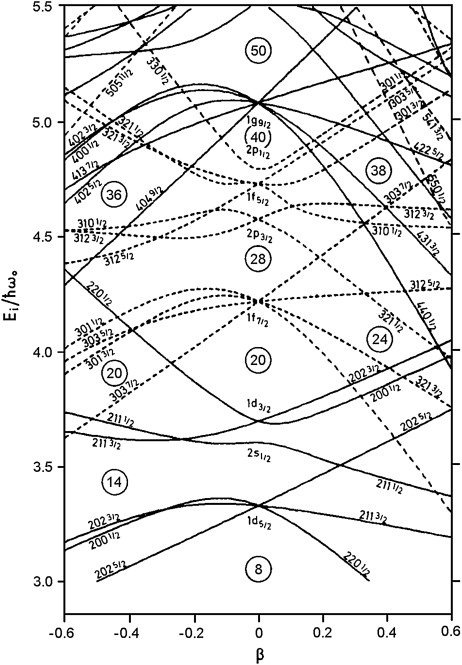
\includegraphics{Introduction_Figs/nilsson.jpg}
    \caption{The Nilsson diagram, showing the evolution of the shell levels of the nucleus with respect to the deformation parameter $\beta$. As the nucleus gets more deformed, the closed shells break down. Taken from \citep{choppin13:_nilsson}.}
    \label{fig:nilsson}
\end{figure}

In the area around $Z=60$ and $N=90$, away from the closed shells, nuclei do not hold a spherical shape. They lose symmetry on the major axes, becoming axially assymmetric via $x=y\neq z$ or $x \neq y \neq z$. The former case has two forms: oblate (pancake-like) or prolate (football-like) depending on whether the nucleus appears compressed (oblate) or elongated (prolate) along the symmetry axis ($z$), as seen in Figure \ref{fig:deformation}. In Figure \ref{fig:nilsson}, the negative $\beta$ corresponds to oblate nuclei, while positive $\beta$ corresponds to prolate nuclei. There are more exotic deformations when the latter assymmetry is true, where symmetry is broken along two or more axes, resulting in pear-shapes and other exotic formations.

\begin{figure}
    \centering
    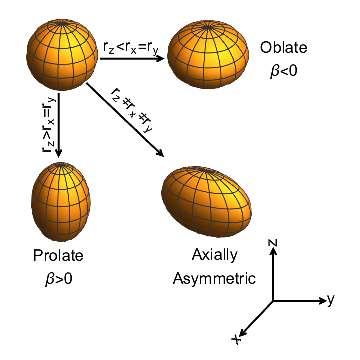
\includegraphics[scale=0.6]{Introduction_Figs/Deformation.png}
    \caption{Illustration of different kinds of deformation, where spherical symmetry is lost. Treating the vertical as the axis of symmetry, the prolate nucleus is contracted along this axis, but is still axially symmetric. The oblate nucleus is elongated along this axis, but otherwise axially symmetric. It is also possible for the nucleus to lose axial symmetry.}
    \label{fig:deformation}
\end{figure}

There are several ways to look for deformation in a nucleus. The most common is the quadrupole moment, which is directly related to the deformation parameter, $\beta$ by

\begin{equation}
    Q_0 = \frac{3}{\sqrt{5\pi}}ZR_0^2\beta\left(1+0.16\beta\right)
\end{equation}

to second order, where $Z$ is the atomic number, and $R_0$ is the approximate radius based on $R_0=1.2A^{1/3}$fm, where $A$ is the number of nucleons \citep{casten90:_structure}. This can be measured in even-even nuclei using the transition between the first excited $2^+$ state and the $0^+$ ground state. The onset of deformation can be seen in Figure \ref{fig:beta_by_isotope}, via the rapid increase in $\beta_2$, the quadrupole deformation parameter. The equation used to calculate $\beta_2$ for this figure is 

\begin{equation}
    \beta_2 = \frac{4\pi}{3ZR^2_0}\left[B(E2)\right]^{1/2}
\end{equation}

where B(E2) is the reduced transition probability for the $0^+_1\rightarrow2^+_1$ transition. There is no way to distinguish prolate and oblate using this calculation.

\begin{figure}[!]
    \centering
    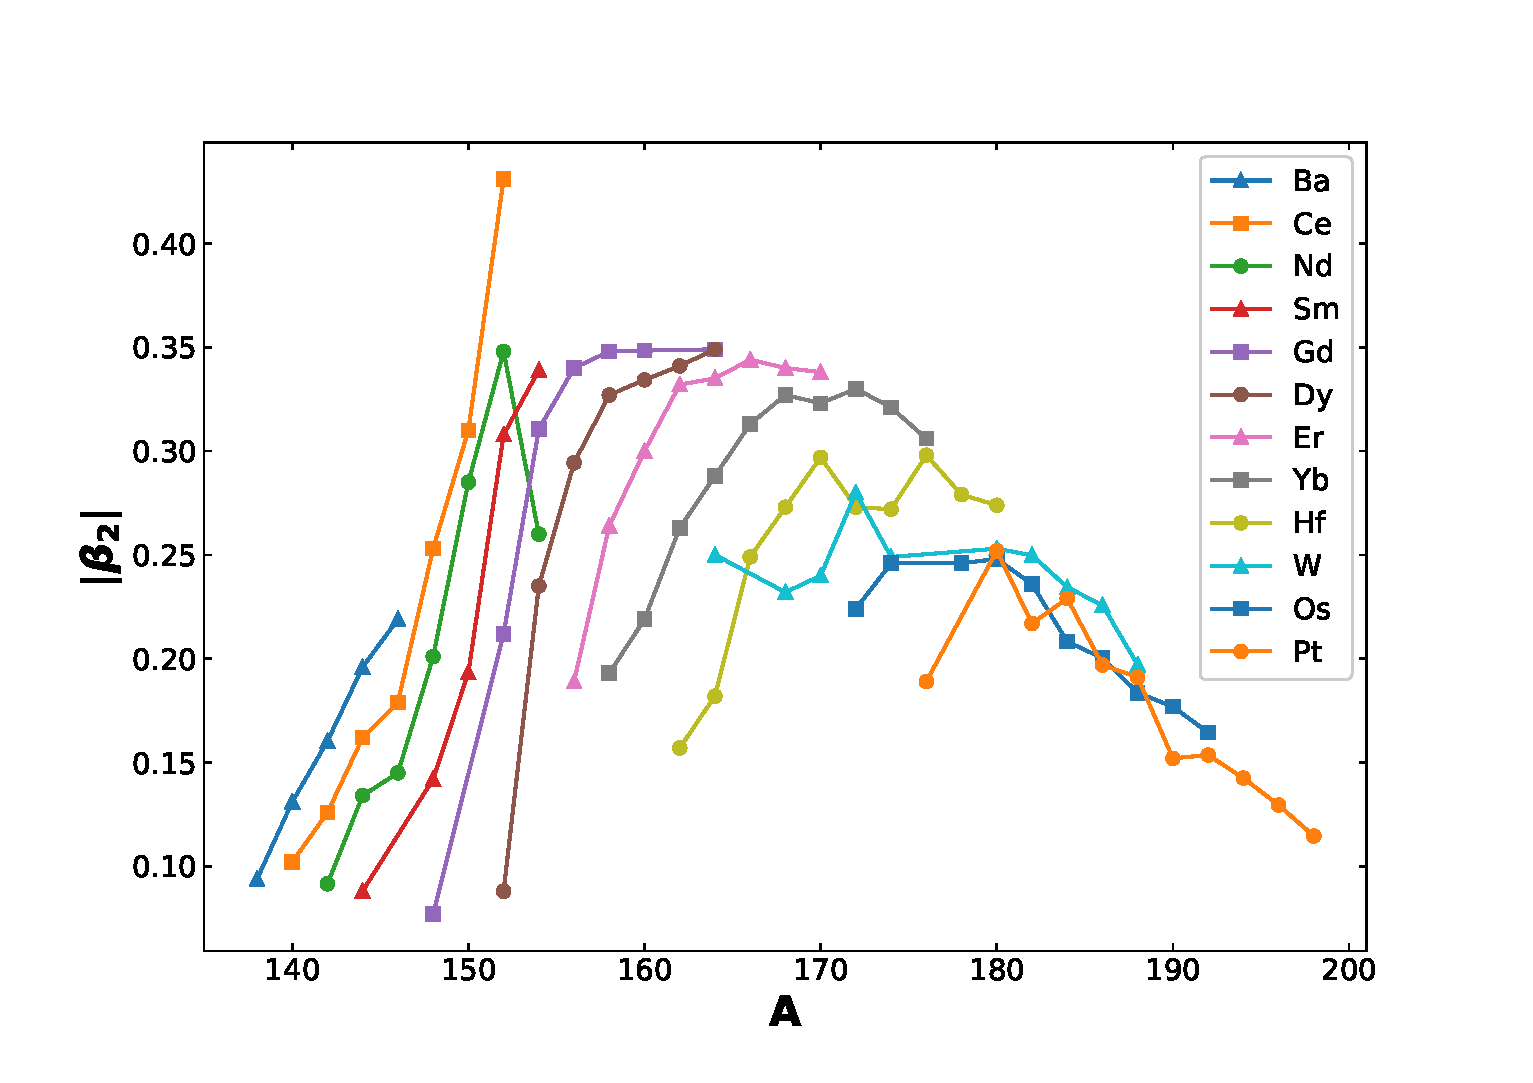
\includegraphics[scale=0.5]{Introduction_Figs/beta.eps}
    \caption{Plot of the norm of the deformation parameter $\beta_2$ along isotopic chains. Deformation can be seen setting in, as isotopic chains transition from spherical to deformed. $\beta_2$ is the quadrupole deformation parameter. The norm of $\beta_2$ is used, as the method used to calculate $\beta_2$ only gives a magnitude, not a sign. A secondary method is needed to distinguish between prolate and oblate.}
    \label{fig:beta_by_isotope}
\end{figure}

In the lanthanide region, there are multiple stable isotopes of several elements, including samarium ($Z=62$) and gadolinium ($Z=64$). Studies across these elements show the onset of deformation through systematics like the energy of the first excited $2^+$ state, and the ratio between the energies of the first $4^+$ and $2^+$ excited states, seen in Figure \ref{fig:E4E2}. The $E_{4^+_1}/E_{2^+_1}$ ratio theoretically tops out at 3.3. This ratio gives a measure of the moment of inertia of the ground-state band of the nucleus, as, for a rigid rotor,

\begin{equation}
    E=\frac{\hbar^2}{2\mathscr{J}_{eff}}J(J+1)
\end{equation}

The moment of inertia, $\mathscr{J}_{eff}$, varies as energy increases. In a perfect rigid rotor, this would not be the case, and $\mathscr{J}_{eff}=\mathscr{J}_{rigid}=\frac{2}{5}Am_{\mathscr{N}}r_0^2A^{2/3}$. Taking the ratio of two energy levels, $J=4$ and $J=2$ in this case, would give a ratio of 10/3, or 3.3. However, if it is not a rigid rotor, this number deviates from 3.3, as the change in the effective moment of inertia changes. The model used by Bohr and Mottelson shows that $\mathscr{J}_{eff}$ is proportional to the square of the deformation parameter, $\beta$ at low deformation, and approaches that of a rigid body at high deformation \citep{bohr55:_deformation}.

\begin{figure}
    \centering
    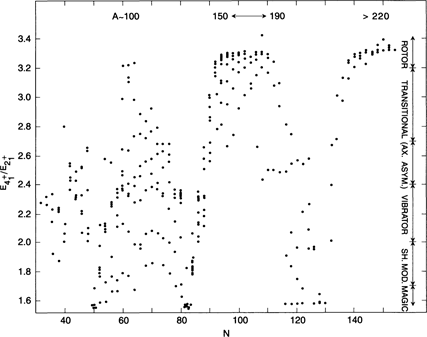
\includegraphics[scale=2]{Introduction_Figs/E4E2RatioCasten.png}
    \caption{Plot of the ratio of the first $4^+$ excited state energy to the first $2^+$ excited state energy in even-even nuclei. On the right, the ratio is broken down into sections, based on structure. This ratio is an excellent diagnostic of the general nuclear structure. Taken from \citep{casten90:_structure}.}
    \label{fig:E4E2}
\end{figure}

Much of these nuclei are successfully modelled with deformation in theoretical calculations \citep{delaroche10:_systematics}. These models can also open up new questions, when a previously identified feature does not fit with the assignment, in an otherwise well described system.

\section{Nuclear Excitations}
\label{sec:nuc_excite}

There are many different ways a nucleus can be excited. While the types of excitations available depend on shape, there are two extremes to consider: a single particle excitation, and a collective excitation. The single particle excitation can be described as a single neutron, proton, or hole from a closed shell being excited to a different level. A collective excitation is usually thought of on a macroscopic level, looking at large numbers of nucleons moving together. These are only extremes, and there are excitations that can be described as multi-particle that would fit in-between. All of these excitations can exist within a nucleus.

\subsection{Collective Excitations}

Two types of collective excitations are rotational and vibrational excitations. Rotational excitations occur in deformed nuclei, as discussed earlier, where spherical symmetry is broken, i.e. $x=y\neq z$ or $x \neq y \neq z$. These are caused by the rotation of the nucleus about the axis of symmetry. Vibrational excitations involve the compression and expansion of the nucleus as a whole. These come in different modes, and have a characteristic even spacing, seen in Figure \ref{fig:statestructure}.

\begin{figure}
    \centering
    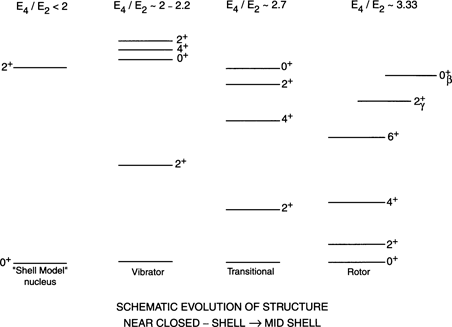
\includegraphics[scale=2]{Introduction_Figs/EvolutionofStructureCasten.png}
    \caption{Cartoon of what excited states built upon different types of nuclei looks like. The closed shell has a large gap between the ground state and first excited state. In the vibrator model, this gap is lower, and a gap of comparable size exists before a cluster of states occurs. In the rotor model, the spacing follows a spacing pattern of $J_f(J_f+1)-J_i(J_i+1)$, with $\gamma$ and $\beta$ vibrations also coming into play. The trasitional area between vibrator and rotor shows a shift between the two, with the clustered states of the vibrator model beginning to space out. Taken from \citep{casten90:_structure}.}
    \label{fig:statestructure}
\end{figure}

There are several ways to tell the difference between these types of excitations. The collective models have well-described spacing of the levels, seen in Figure \ref{fig:statestructure}. Vibrational excitations will be spaced regularly as $n\hbar\omega$, while rotational excitations will have increasing spacing between the levels as $J$ increases. The reduced transition probabilities also give information about the difference between two different levels. The single-particle strengths for these transitions can be calculated and are known as Weisskopf estimates. The reduced transition probability can then be written in Weisskopf units using the estimate, which gives a measure of the collectivity of the transition. This does have limitations, however, as the Weisskopf estimate assumes a spherical nuclear model.

\subsection{Shape Coexistence}

Another aspect of nuclear shape is that of shape coexistence. In shape coexistence, there is more than one minima of the potential well, at different forms of deformation, as illustrated in Figure \ref{fig:shape}. These two minima represent two different shapes of the nucleus, and both can have excitations built upon them. The two shapes can also interact, causing shape mixing effects. 

\begin{figure}[t]
    \centering
    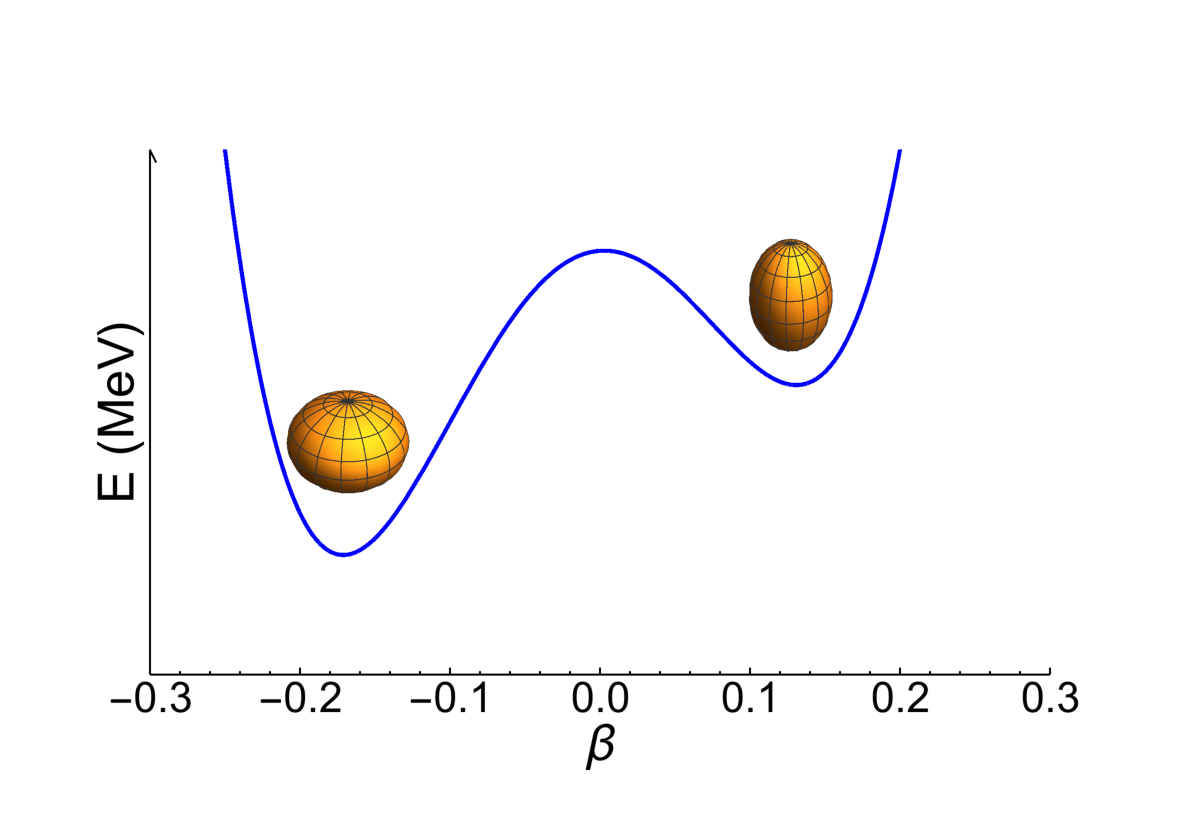
\includegraphics[scale=0.7]{Introduction_Figs/ShapeCoexist.pdf}
    \caption{Cartoon of the potential well of a nucleus with shape coexistence. A second minima appears at a different $\beta$, the deformation parameter. Both of these minima can have excitations built on top of them, leading to shape coexistence. A representation of the shape at $\beta$ is shown in each minima.}
    \label{fig:shape}
\end{figure}

There are two main theoretical approaches to shape coexistence in nuclei: microscopic shell-model and mean-field descriptions \citep{heyde11:_shape_coexist}. These two approaches compliment each other. In the shell-model approach, a spherical shell model is assumed, and particle-hole excitations across closed shells are examined. For an $n$p-$n$h configuration, it would appear the $0^+$ states are too high. However, upon correcting for monopole interaction energy, and then coupling different $n$p-$n$h subspaces together, lower energy $0^+$ states are calculated \citep{caurier07:_shape_coexist}. For calculations above $A=80$, nucleons must be treated in pairs built from realistic collective pairs, as the model spaces become too large for current computational power\citep{heyde11:_shape_coexist}. In this approach, intruder states from even-evn particle-hole excitations can create shape-coexisting $0^+$ states.

The mean-field approach uses the self-consistent Hartree-Fock-Bogoliubov (HFB) theory. The effective forced are tuned to describe global nuclear properties. When minimizing the energy, deformation in the nuclear shape can result. Various mean-field states are found, which have broken symmetries needed witin the nucleus. These states are projected onto the proper particle numbers, isospin, and angular momentum to produce the physical states observed \citep{heyde11:_shape_coexist}. To compare with experimental date, the Hamiltonian must be rediagonlized in terms of the physical, projected states.

This shape coexistence, like the collective excitations, have spectroscopic fingerprints that can help determine their existence. As with deformation, large reduced transition rates are a possible sign of shape coexistence, but do not distinguish between static and dynamic deformation \citep{heyde11:_shape_coexist}. The diagonal $E2$ matrix elements can distinguish between the dynamic and static. The $E0$ transitions present in $J^{\pi}\rightarrow J^{\pi}$ may also be an indirect fingerprint of shape coexistence, as it is related to the change in the mean radius of the nucleus, as discussed in section \ref{sec:E0}\citep{wood99:_e0}. The low-lying states of interest can be difficult to observe, as they are not populated strongly in reactions.

\section{Multipole Radiation}
\label{sec:multipole}
When the nucleus is in an excited state, with energy in excess of its ground state, this excess is stored in the protons and neutrons of the nucleus. These nuclei oscillate, creating electromagnetic fields with their oscillation. The nucleus is then capable of deexciting in different ways, including photon emission in the form of $\gamma$-rays, the carrier of the electromagnetic force. These fields are commonly described using expansions of spherical harmonics, allowing for angular momentum identification of the radiation emitted. This expansion is commonly referred to as multipole expansion. Discussion and derivation can be found in detail in many references \citep{blatt79:_emradiation, jackson99:_emradiation, zangwill13:_emradiation}.

The Maxwell equations are
\begin{subequations}
\label{eq:maxwell_free}
\begin{align}
    \nabla \cdot \textbf{E} & = 0 &   \nabla \times \textbf{E} & = -\frac{\partial \textbf{B}}{\partial t} \\
     \nabla \cdot \textbf{B} & = 0 &  \nabla \times \textbf{B} & = \frac{1}{c^2}\frac{\partial \textbf{E}}{\partial t}
\end{align}
\end{subequations}
for a vacuum with no source. Radiation from a nuclear transition has a well-defined energy, and therefore, a well-defined frequency $\omega$. The time-dependence of the electric and magnetic field can be expressed as
\begin{subequations}
\label{eq:maxwell_rad}
\begin{align}
    \textbf{E}(\textbf{r},t) & = Re\left\{\textbf{E}(\textbf{r},t)e^{-i\omega t}\right\} \\
    \textbf{B}(\textbf{r},t) & = Re\left\{\textbf{B}(\textbf{r},t)e^{-i\omega t}\right\}
\end{align}
\end{subequations}
 
Using equations \ref{eq:maxwell_free} and \ref{eq:maxwell_rad}, the Maxwell equations can be rewritten in the equivalent forms
\begin{subequations}
\label{eq:maxwell_rw1}
\begin{gather}
    \left(\nabla^2+k^2\right)\textbf{E} = 0 \\
    \nabla \cdot \textbf{E} = 0 \\
    \textbf{B}=-\frac{i}{ck} \nabla \times \textbf{E}
\end{gather}
\end{subequations}
and
\begin{subequations}
\label{eq:maxwell_rw2}
\begin{gather}
    \left(\nabla^2+k^2\right)\textbf{B} = 0 \\
    \nabla \cdot \textbf{B} = 0 \\
    \textbf{E}=-\frac{ic}{k} \nabla \times \textbf{B}
\end{gather}
\end{subequations}

As these are equivalent, any pair of fields \textbf{B}(\textbf{r}) and \textbf{E}(\textbf{r}) that satisfy equations \ref{eq:maxwell_rw1} must satisfy equations \ref{eq:maxwell_rw2} and vice-versa. It can be shown that any arbitrary solution to the Maxwell equations can be written as a linear combination of a transverse magnetic wave and a tranverse electric wave, i.e. 
\begin{align}
    \label{eq:trans_E}
    \textbf{r} \cdot \textbf{E} & = 0, \text{ or} \\
    \label{eq:trans_B}
    \textbf{r} \cdot \textbf{B} & = 0
\end{align}

When combining \ref{eq:trans_E} and \ref{eq:maxwell_rw1}, a solution to the Maxwell equations can be derived. When doing the same with \ref{eq:trans_B} and \ref{eq:maxwell_rw2}, a separate, linearly independent, solution can be derived. These two solutions in combination can express any of the solutions to the Maxwell equations as a linear combination.

Because of the linear independence of the spherical harmonics, solutions to these wave equations can be written as multipole expansions, the term multipole in reference to the angular momentum, $l$, defining the series of the harmonic. The first set of solutions give the magnetic multipole fields, with the solutions
\begin{subequations}
\label{eq:magnetic_sol}
\begin{align}
    \left(\nabla^2+k^2\right)\textbf{E}^\text{M} & = 0 & \textbf{B}^\text{M}=-\frac{i}{ck} \nabla \times \textbf{E}^\text{M} \\
    \nabla \cdot \textbf{E}^\text{M} & = 0 & \textbf{r}\cdot\textbf{E}^\text{M}=0
\end{align}
\end{subequations}
where the M indicates the magnetic multipole component of the field. Second set give the electric multipole fields with the solutions
\begin{subequations}
\label{eq:electric_sol}
\begin{align}
    \left(\nabla^2+k^2\right)\textbf{B}^\text{E} & = 0 & \textbf{E}^\text{E}=-\frac{ic}{k} \nabla \times \textbf{B}^\text{E} \\
    \nabla \cdot \textbf{B}^\text{E} & = 0 & \textbf{r}\cdot\textbf{B}^\text{E}=0
\end{align}
\end{subequations}
where the E indicates the electric multipole component of the field. The total fields are then just the two components summed together.

These multipole fields can be written as an expansion of the spherical Hankel functions, $h_l^{1,2}(kr)$, multiplied by the spherical harmonics, $Y_{lm}(\theta,\phi)$. The fields can then be broken apart into components of $l$, the angular momentum.  The general expressions for $\textbf{E}^\text{M}$ and $\textbf{B}^\text{E}$ fields are
\begin{subequations}
\begin{align}
    \textbf{E}^\text{M}(\textbf{r})=\sum_{l,m,i}c_{lm}^{(i)}h_l^{(i)}\textbf{l}Y_{lm}(\theta,\phi) \\
    \textbf{B}^\text{E}(\textbf{r})=\sum_{l,m,i}d_{lm}^{(i)}h_l^{(i)}\textbf{l}Y_{lm}(\theta,\phi)
\end{align}
\end{subequations}
with $\textbf{E}^\text{E}$ and $\textbf{B}^\text{M}$ derivable from the curl expressions in \ref{eq:maxwell_rw1} and \ref{eq:maxwell_rw2}. In this equation, the orbital angular momentum is expressed as $\textbf{l}=-i(\textbf{r}\times\nabla)$ The created multipole radiation of E and M types, being listed as E$l$ and M$l$ radiation. Then the vector spherical harmonics can be introduced in the form
\begin{equation}
    \textbf{X}_{lm}=\frac{1}{\sqrt{l(l+1)}}\textbf{l}Y_{lm}(\theta,\phi)
\end{equation}
A further simplification can be defined as
\begin{equation}
    f_{lm}(kr)=a_{lm}^{(1)}h_l^{(1)}(kr)+a_{lm}^{(2)}h_l^{(2)}(kr)
\end{equation}
leading to
\begin{subequations}
\begin{align}
    \textbf{B}_l^\text{E}(\textbf{r}) & = \sum_m f_{lm}^{\text{E}}(kr)\textbf{X}_{lm}(\theta,\phi) & \textbf{E}_l^\text{M}(\textbf{r}) & = \sum_m f_{lm}^{\text{M}}(kr)\textbf{X}_{lm}(\theta,\phi)\\
    \textbf{E}_l^\text{E}(\textbf{r}) & = -\frac{ic}{k}\nabla\times \textbf{B}_l^\text{E}(\textbf{r}) & \textbf{B}_l^\text{M}(\textbf{r}) & = -\frac{i}{ck}\nabla\times \textbf{E}_l^\text{M}(\textbf{r})
\end{align}
\end{subequations}
With these definitions, the total electric and magnetic fields of can be written as
\begin{subequations}
\begin{align}
    \textbf{E}(\textbf{r}) & = \sum_{l=1}^{\infty}\sum{m=-l}^{l} a^\text{E}(l,m)\textbf{E}^\text{E}(l,m;\textbf{r})+ a^\text{M}(l,m)\textbf{E}^\text{M}(l,m;\textbf{r}) \\
    \textbf{B}(\textbf{r}) & = \sum_{l=1}^{\infty}\sum{m=-l}^{l} a^\text{E}(l,m)\textbf{B}^\text{E}(l,m;\textbf{r})+ a^\text{M}(l,m)\textbf{B}^\text{M}(l,m;\textbf{r}) 
\end{align}
\end{subequations}
These amplitudes $a^\text{E}$ and $a^{M}$ can be derived \citep{blatt79:_emradiation}. They come out to be
\begin{subequations}
\begin{align}
    a^\text{E}(l,m) \simeq - \frac{4\pi}{(2l+1)!!}\left(\frac{l+1}{l}\right)^{1/2}\kappa^{l+2}(Q_{lm}+Q'_{lm}) \\
    a^\text{M}(l,m) \simeq + \frac{4\pi}{(2l+1)!!}\left(\frac{l+1}{l}\right)^{1/2}\kappa^{l+2}(M_{lm}+M'_{lm})
\end{align}
\end{subequations}
where $\kappa\equiv\omega/c$, the wave number. Then, using the charge distribution, $\rho(\textbf{r})$, and magnetic distribution $\textbf{M}(\textbf{r})$, and current distribution $\textbf{j}(\textbf{r})$ we define
\begin{subequations}
\label{eq:multipole_moment}
\begin{align}
    Q_{lm} & = \int r^l Y_{lm}^*(\theta,\phi)\rho(\textbf{r})dV \\
    Q'_{lm} & = -\frac{i\kappa}{l+1}\int r^l Y_{lm}^*(\theta,\phi)\nabla(\textbf{r}\times\textbf{M})dV \\
    M_{lm} & = -\frac{1}{c(l+1)}\int r^l Y_{lm}^*(\theta,\phi)\nabla(\textbf{r}\times\textbf{j})dV \\
    M'_{lm} & = -\int r^l Y_{lm}^*(\theta,\phi)\nabla\textbf{M}dV
\end{align}
\end{subequations}
These are the electric ($Q_{lm}$ and $Q'_{lm}$) and magnetic ($M_{lm}$ and $M'_{lm}$) multipole moments. To use them for nuclear transitions, the distributions must take the initial and final states into account. They become
\begin{subequations}
\begin{align}
    \rho(i,f;\textbf{r}) & = e \varphi_f^*(\textbf{r})\varphi_i(\textbf{r}) \\
    \textbf{M}(i,f;\textbf{r}) & = \frac{e\hbar}{2Mc}\mu\left\{\varphi_f^*\boldsymbol{\sigma}\varphi_i\right\} \\
    \textbf{j}(i,f;\textbf{r}) & = \frac{e}{2M}\left[\varphi_f^*(\textbf{p}\varphi_i)+(\textbf{p}\varphi_f)^*\varphi_i\right]
\end{align}
\end{subequations}
where $M$ and $e$ are the mass and charge of a single particle, $\textbf{p}=i\hbar\nabla$ is the linear moment operator, $\mu$ is the magnetic moment in Bohr magnetons, and $\boldsymbol{\sigma}$ is the Pauli spin operator.

From here, it is possible to obtain the transition probability using Fermi's golden rule,
\begin{equation}
    \label{eq:golden}
    w_{if}=\frac{2\pi}{\hbar}\abs{\bra{f}H_{int}\ket{i}}^2\rho,
\end{equation}
where $H_{int}$ is the interaction Hamiltonian from the generated field. This Hamiltonian is
\begin{equation}
    H = -\frac{1}{c}\boldsymbol{A}\cdot\mathcal{J}
\end{equation}
where $\mathcal{J}$ is the current density and $\boldsymbol{A}$ is the magnetic vector potential, which can be derived from the solutions above \citep{wong90:_nuclear}. Combining all of this together with Fermi's golden rule, the transition probabilities are
\begin{subequations}
\begin{align}
    T^\text{E}(l,m) & = \frac{8\pi(l+1)}{l[(2l+1)!!]^2}\frac{\kappa^{2l+1}}{\hbar}\abs{Q_{lm}+Q'_{lm}}^2 \\
    T^\text{M}(l,m) & = \frac{8\pi(l+1)}{l[(2l+1)!!]^2}\frac{\kappa^{2l+1}}{\hbar}\abs{M_{lm}+M'_{lm}}^2
\end{align}
\end{subequations}

Of note from this derivation, the transition probability decreases with increasing $l$, making lower angular momentum transitions more favorable. Additionally, looking at the multipole moments, once the wave equations have been added in, all but $Q_{lm}$ have a factor of $1/c$. This makes the electric transition stronger than the magnetic transition of the same $l$.

There are limitations for the types of multipole radiation that can be emitted due to a transition, known as selection rules. One such limitation is that all of the multipole moments of equations \ref{eq:multipole_moment} go to zero is $l=0$, making $l=0$ transitions forbidden via this method. Other rules are based on two pieces of information about the initial and final states: the spins and parities of the states. The spins, $J$ of the states select the allowable $l$, using the range $\abs{J_i-J_f}\leq l\leq J_i+J_f$, meaning the change in angular momentum cannot exceed the sum of the spins of the two states, or be smaller than the difference of the spins of the two states. For example, a transition between two states of spins 4 and 2 would allow $l$ from 2 to 6. The parity selection now helps select the set of solutions. With the first selection rule, in the example, the possibilities are E2, M2 ... E6, M6. If the parity stays the same between the two states, so positive to positive or negative to negative, the solutions are even E$l$ and odd M$l$. If the parity changes, the solutions are odd E$l$ and even M$l$. In an equation form, the parity change is
\begin{align}
    \pi(\text{E}l) &= (-1)^{l} & \pi(\text{M}l) &= (-1)^{l-1}
\end{align}

While not a selection rule, multipoles of lower order are stronger, and electric multipoles are stronger than magnetic multipoles, with M$l$ having about the same intensity as E$l+1$. There are also forbidden transitions to consider. The name is a misnomer, as these transitions are not strictly forbidden, but are highly suppressed, or must occur through a different mechanism. A relevant example to this text is that of the $l=0$ transition, previously noted as forbidden. Photons carry an angular momentum of 1, so any transitions that occur via photon emission must have a $\delta J \geq 1$, so $l$ must be at least 1. An E0 transition has $l=0$, making it forbidden by single photon emission. However, it can still occur, several different ways.

\section{Internal Conversion}

In an excited state, the nucleus has several ways of decaying, the previously discussed photon emission being only one. In a highly excited state, above the binding energy of the nucleus, particle emission can occur, changing the makeup of the nucleus. In cases where particle emission is forbidden, electromagnetic radiation deexcites the nucleus. Above 1.022 MeV of excitation, the nucleus can also deexcite via pair-production, the creation of an electron-positron pair. Below this energy, there are two processes to deexcite the nucleus: photon emission and internal conversion. Photon emission was discussed above in section \ref{sec:multipole}. Internal conversion occurs internally within the atom, with the excitation energy being transfer to an orbiting atomic electron. The electron is then ejected from its bound state, as the energy it has been given exceeds the electron binding energy, giving the electron a kinetic energy of 
\begin{equation}
    T_e = E_{\gamma}-BE
\end{equation} 
where $BE$ is the atomic binding energy of the electron, and $E_{\gamma}$ is the transition energy. The electron carries information about the multipolarity of the transition it was ejected from, as a photon would if emitted for the same transition.

Both of these processes come from the same overall mechanism, that of the electromagnetic field, but internal conversion also has a component from the nuclear interaction. As a result, internal conversion can be described with the conversion coefficient
\begin{equation}
\label{eq:conv_coeff}
    \alpha = \frac{w_e}{w_\gamma}
\end{equation}
where $w_e$ is the transition probability due to internal conversion and $w_\gamma$ is the transition probability due to single photon emission.

Internal conversion is a result of the interaction of the electron's wavefunction with that of the nucleus. The probability for internal conversion can be derived using Fermi's Golden rule, equation \ref{eq:golden}, where $H_{int}$ is the electromagnetic interaction of the combined initial nuclear and electron states, to the combined final nuclear state and free electron, and $\rho$ is the accessible energy state density for the ejected electron. For simplicity, this derivation will be specifically for $K$ electrons, and look at the area outside of the nuclear radius \citep{roy67:_e0, blatt79:_emradiation, segre77:_icradiation}.

The electron can be treated as a plane wave once it has been ejected from the $K$ shell, assuming the electron energy is large compared to the binding energy. This makes the initial and final states of the electron
\begin{subequations}
\begin{align}
    \psi_{i} & = \left(\pi\left(\frac{a_0}{Z}\right)^3\right)^{-1/2}e^{-\frac{RZ}{a_0}}\\
    \psi_{f} & = V^{-1/2}e^{i\textbf{k}\cdot\textbf{R}}
\end{align}
\end{subequations}
where $a_0=\hbar^2/me^2$ is the Bohr radius of the hydrogen atom, \textbf{R} is the position vector between the electron and the center of the nucleus, \textbf{k} us the wave vector of the electron after ejection, and $V$ is the volume of the "box", which should drop out in the final result, as $\rho$ also contains the volume in its formulation. The energy state density can be rewritten in terms of the wave vector \textbf{k} to be 
\begin{align}
    \rho & = z(k)d\Omega, \text{ where} \\
    z(k) & = V\frac{m\hbar k}{(2\pi\hbar)^3}
\end{align}
Taking into account there are two electrons in the $K$-shell, the probability $w_{if}$ can then be rewritten as
\begin{equation}
\label{eq:golden_ic}
    w_{if}=2 \frac{2\pi}{\hbar}z(k)\int\abs{\bra{f}H_{int}\ket{i}}^2d\Omega
\end{equation}

For this derivation, the electric multipoles are being considered, so only the electrostatic interaction is being used. By using the magnetic interaction instead, the magnetic multipoles can also be derived. By assuming the interaction is occurring outside of the nucleus, the Hamiltonian can be assumed to be the electrostatic interaction between the protons of the nucleus and the electron or
\begin{equation}
    H=\sum_{i=1}^Z \frac{e^2}{\abs{\textbf{R}-\textbf{r}_i}}
\end{equation}
where \textbf{R} is as described above, and $\textbf{r}_i$ is the proton position from the center of the nucleus. Then the matrix element is
\begin{equation}
\label{eq:matrix_element_int}
    \abs{\bra{f}H_{int}\ket{i}} = \left(V\pi\left(\frac{a_0}{Z}\right)^3\right)^{-1/2}\int e^{-i\textbf{k}\cdot\textbf{R}}\varphi_{f}^* \frac{e^2}{\abs{\textbf{R}-\textbf{r}_i}} e^{-\frac{RZ}{a_0}}\varphi_{i}d\Omega
\end{equation}
with $\varphi_{i}$ and $\varphi_{f}$ being the initial and final wave functions of the nucleus, respectively. The integration must occur over both the coordinates of the electron and over the coordinates in the nuclear wave functions, such that $d\Omega=d^3Rd\tau$ where $\tau$ represents the nuclear coordinates.

The main contribution to the integral is going to come from $\textbf{R}>\textbf{r}_i$, the earlier assumption the interaction is occurring outside of the nucleus. This allows for an expansion of $\abs{\textbf{R}-\textbf{r}_i}^{-1}$ in terms of spherical harmonics such that
\begin{equation}
\label{eq:expansion_Rri}
    \frac{1}{\abs{\textbf{R}-\textbf{r}_i}} = \sum_{l=0}^\infty\sum_{m=-l}^{l}\frac{4\pi}{2l+1}\frac{r_i^l}{R^{l+1}}Y_{lm}(\Theta,\Phi)Y_{lm}^{*}(\theta_i,\phi_i)
\end{equation}
where $\Theta$ and $\Phi$ are the polar vector of \textbf{R} and $\theta_i$ and $\phi_i$ are the same for $\textbf{r}_i$. Substituting this into equation \ref{eq:matrix_element_int} gives
\begin{equation}
    
    abs{\bra{f}H_{int}\ket{i}} = \frac{e}{ \left(V\pi\left(\frac{a_0}{Z}\right)^3\right)^{1/2}} \sum_{l=0}^\infty\sum_{m=-l}^{l}\frac{4\pi}{2l+1} Q_{lm}(i,f)J_{lm}
\end{equation}
where $Q_{lm}(i,f)$ is the electric multipole matrix element and $J_{lm}$ is the integral
\begin{equation}
    J_{lm}\equiv\int e^{-\frac{RZ}{a_0}}e^{-i\textbf{k}\cdot\textbf{R}}R^{-(l+1)}Y_{lm}(\Theta,\Phi)d^3R
\end{equation}
Because of the earlier assumption of the outgoing electron being a plane wave by assuming the energy is sufficiently large, such that $ka_0/Z\gg1$. With this approximation, $e^{-\frac{RZ}{a_0}}\simeq1$ and the integral can be evaluated. Treating $\theta$ and $\phi$ as polar angles for \textbf{k}, 
\begin{equation}
    J_{lm}=4\pi i^{-l}\frac{k^{l-2}}{(2l-1)!!}Y_{lm}(\theta,\phi)
\end{equation}

Substituting all of this into \ref{eq:golden}, the transition probability is
\begin{equation}
    w_{if}=128\pi\frac{me^2Z^3}{\hbar^2a_0^3} \sum_{l=0}^\infty\sum_{m=-l}^{l} \frac{k^{2l-3}}{\left[\,(2l-1)!!\right]\,^2}\abs{Q_{lm}(i,f)}^2
\end{equation}
There is a strong dependence on atomic number $Z$ and the multipole order $l$. The magnetic transition follows a similar derivation, with a solution distinct from the electric one just derived. Thus, measuring the conversion coefficient of a transition can be used to determine the multipolarity of the transition. The theoretical $K$-shell conversion coefficients for $l=1,2,3$ are plotted in Figure \ref{fig:icc_gd} for comparison.

\begin{figure}
    \centering
    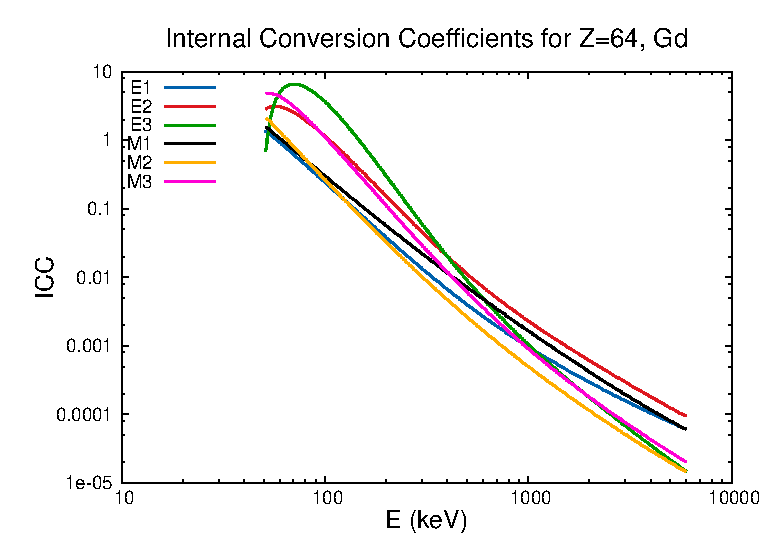
\includegraphics[scale=1]{Introduction_Figs/ICCGd.eps}
    \caption{The theoretical K-shell conversion coefficients for the magnetic and electric multipoles for $l=1,2,3$, calculated using BrICC \citep{kibedi08:_BRICC}. Each of the multipoles is distinct. Further distinction between multipoles can be seen by plotting the intensity ratios between different electronic shells.}
    \label{fig:icc_gd}
\end{figure}.

\subsection{E0 Transitions}
\label{sec:E0}

Like the electromagnetic radiation, $l=0$ transitions are still forbidden in the internal conversion proof above, as the rate directly depends on $Q_{lm}$, which goes to 0 for $l=0$, which is relevant to transitions where the initial and final spins are the same. This, however, arises from the previous assumption of looking only outside of the nucleus. While the majority of the interaction between nucleus and electron occurs outside of the nucleus, when this goes to zero, as is the case for $l=0$, the correction term from inside the nucleus must be taken into account, i.e. $R<r_i$. This exchanges the positions of $R$ and $r_i$ on the right in the expansion from equation \ref{eq:expansion_Rri}. Revisiting equation \ref{eq:matrix_element_int}, and setting $l=0$ it becomes
\begin{equation}
\label{eq:matrix_element_E0}
    \abs{\bra{f}H_{int}\ket{i}} = \frac{e}{\left(V\pi\left(\frac{a_0}{Z}\right)^3\right)^{1/2}}\sum_{i=1}^Z \int d\tau\varphi_{f}^*\frac{1}{r_i}\varphi_{i} \int_{R<r_i}d^3R e^{-i\textbf{k}\cdot\textbf{R}} e^{-\frac{RZ}{a_0}}
\end{equation}
As integration over R extends only to very small numbers, the exponentials on the right can be approximated as 1, simplifying the integral to just $d^3R$, making it $4\pi r_i^3/3$. The matrix element is now
\begin{equation}
\label{eq:hint_e0}
    \abs{\bra{f}H_{int}\ket{i}} =  \frac{4\pi}{3}\frac{e}{\left(V\pi\left(\frac{a_0}{Z}\right)^3\right)^{1/2}} \sum_{i=1}^Z \int d\tau\varphi_{f}^*r_i^2\varphi_{i}
\end{equation}
The sum is of the order of magnitude of the square of the nuclear charge radius, denoted by $\mathcal{R}^2$. Substituting \ref{eq:hint_e0} into \ref{eq:golden_ic}, the probability for an electric multipole of order $l=0$ becomes
\begin{equation}
    w_{if} = \frac{32}{9}\frac{e^2}{\hbar c}Z^3\left(\frac{\mathcal{R}^2}{a_0^2}\right)^2\left(2\frac{\Delta E}{mc^2}\right)^{1/2}\frac{mc^2}{\hbar}
\end{equation}
where $\Delta E=E_f-E_i-B_K$ is the energy of the electron, with $B_K$ indicating the atomic binding energy of the $K$-shell. At first glance, this indicates the $l=0$ (E0) component is a measure of the change in the nuclear charge radius. The diagonal components of the E0 operator are measures of the mean-square charge radius \citep{wood99:_e0}. The off-diagonal terms, which would be the terms probed by conversion electron spectroscopy are a direct probe of the nuclear dynamic. The interpretation of E0 components does not have a complete consensus \citep{ilie11:_deformed}.

One common way to rewrite the E0 transition probability is 
$\mathcal{W}=\Omega\rho^2$, where $\Omega$ are non-nuclear factors, i.e. $\Omega=\sum_i\Omega_i$ where $i$ is the electron shell. This contains the nuclear factors to $\rho^2$, referred to as the nuclear strength parameter \citep{church56:_monopole,wood99:_e0}. In practice, $\rho^2$ tends to fall between $10^{-1}-10^{-3}$, so it is standard to quote $\rho^2\times10^3$. For a given transition, \begin{equation}
    \rho^2_{if}=\abs{\frac{\bra{f}\sum_ke_kr_k^2\ket{i}}{eR^2}}^2
\end{equation}
This makes $\rho^2$ unitless, due to the division by $eR^2$, where $R$ is the standard nuclear radial approximation. With this, $\rho^2$ can be scaled in terms of mass, allowing for comparisons across the nuclear chart \citep{wood99:_e0}.

These transitions have been seen to manifest via a variety of phenomena, including the shell model, collective models, shape mixing i.e. shape coexistence and intruder states\citep{wood99:_e0}. Depending upon which phenomenon is responsible for a given E0 transition will change $\rho^2$, of which estimates can be calculated. many of these models lead to small E0 rates, the exception being shape mixing. Due to the dominant nature of shape mixing in E) decays, it is difficult to compare these models with experimental $\rho^2$ values unless shape-mixing effects have been removed \citep{wood99:_e0}.

\section{The Rare Earth Region: $N=90,Z=60$}

The region around $N=90,Z=60$ is far away from the closed shells, and constitutes the largest region of deformed nuclei in the chart of nuclides. This region of nuclei has a variety of interesting structure features that are not fully characterized, including a large number of bound $0^+$ states outside of the ground state \citep{meyer06:_zeroplus}. Many of these states have not been fully characterized, including gamma-spectroscopy, electron-spectroscopy and lifetime measurements. With this large number of $0^+$ states, electron-spectroscopy becomes vital, as transitions between two $0^+$ states must be E0 in nature, which cannot occur via gamma radiation.

The isotopic chains of the rare earth region can be seen plotted against the magnitude of the deformation parameter $\beta$ in Figure \ref{fig:beta_by_isotope}. There is a large amount of deformation in the region, and several isotopes with large numbers of $0^+$ states, including $^{152}$Gd, $^{156}$Gd, $^{162}$Dy, and $^{168}$Er, all of which have more than 10 $0^+$ states below 3 MeV \citep{meyer06:_zeroplus}, with $^{154}$Gd having the most, at 16 states. In addition, $^{158}$Gd also has a large number of $0^+$ states at 13 \citep{lesher02:_158gd}. This makes the Gd isotopic chain excellent for studying the nature of these excited $0^+$ states in deformed nuclei.

In section \ref{sec:nuc_excite}, collective excitations and shape coexistence were discussed. In these deformed nuclei, there are a large number of collective excitations, the nature of which is unknown. E0 transitions in the region have been seen to have large transition strengths, and have been associated with shape coexistence \citep{wood99:_e0}. Confirming shape coexistence cannot be done with a single measurement. With the large number of $0^+$ states present in this region of the nuclear chart, E0 strengths become a vital spectroscopic fingerprint in interpretation and understanding \citep{heyde11:_shape_coexist}. These transitions give a model-independent view of the configurations underlying the transition. Fully understanding the $0^+$ states in nuclei will require a systematic study of E0 transition strengths including those from $\Delta J\neq0$.